% Simple poster (portrait)
% Author: Sofia Jijon (https://sjijon.github.io)
% Last Update: Sept 9, 2021
% Latest Version: https://github.com/sjijon/TeX-templates/tree/main/Tikzposter%20posters/Simple%20poster

\documentclass[a0paper,portrait,margin=0pt, colspace=24pt,subcolspace=0pt,blockverticalspace=36pt,innermargin=50pt]{tikzposter}

\usepackage[latin9]{inputenc}
\usepackage[square,numbers]{natbib} 	% Bibliography manager
\usepackage{amsmath,amssymb}
\usepackage{lipsum}  				    % Random Text
\usepackage[colalign]{aligncolsatbottom}  %To align columns at bottom (!! please run 2 times)

%..............................................................................................................................................................................................
% Display
\tikzposterlatexaffectionproofoff 			
\usetikzlibrary{shapes.geometric,arrows.meta,positioning}  %Tikz Libraries

% Fonts
\usepackage{helvet}					% Sans-Serif
\renewcommand{\familydefault}{\sfdefault}	%

% Colors
	\definecolor{MyOrange}{rgb}{0.8, 0.33, 0}
	\definecolor{MyBrown}{rgb}{0.28, 0.20, 0.20}
	\definecolor{MyGreen}{rgb}{0.33, 0.42, 0.18}

% Theme
\usetheme{Default}
\definecolorstyle{MyStyle2016}{
	\definecolor{ColorOne}{named}{MyBrown} 
	\definecolor{ColorTwo}{named}{MyOrange}
	\definecolor{ColorThree}{named}{MyGreen}
}{
    % Title Colors
    \colorlet{titlebgcolor}{ColorOne}
    \colorlet{titlefgcolor}{white}
    % Background Colors
    \colorlet{backgroundcolor}{ColorOne!15}
    \colorlet{framecolor}{ColorOne}
    % Block Colors
    \colorlet{blocktitlebgcolor}{white}
    \colorlet{blocktitlefgcolor}{ColorTwo}
    \colorlet{blockbodybgcolor}{white}
    \colorlet{blockbodyfgcolor}{black}
    % Innerblock Colors
    \colorlet{innerblocktitlebgcolor}{ColorOne!15}
    \colorlet{innerblocktitlefgcolor}{black}
    \colorlet{innerblockbodybgcolor}{ColorOne!15}
    \colorlet{innerblockbodyfgcolor}{black}
    % Note colors
    \colorlet{notebgcolor}{ColorTwo!20}
    \colorlet{notefgcolor}{ColorTwo}
    \colorlet{notefrcolor}{ColorTwo}
 }

% Color style
\usecolorstyle{MyStyle2016}
%..............................................................................................................................................................................................
\title{Modelling A Limb Congruency Learning Task}

\author{Antonio Amaddio}

\institute{FU-Berlin, Department of Psychology}

%..............................................................................................................................................................................................
\begin{document}
%
%
%	HEAD
%
%....................................................................................
%
%	Title
%
\maketitle[width=0.96\linewidth,titletoblockverticalspace=36pt,linewidth=0,roundedcorners=10]
%..............................................................................................................................................................................................
%
%	LEFT COLUMN
%
\begin{columns}
\column{0.33}
%....................................................................................
%
%	Block
%
\block[titleleft,roundedcorners=16]{1. Research Question}{
	\raggedright
	Is learning of motor actions (finger movement task) moderated by congruency in visual perception?
}
%....................................................................................
%
%	Block
%
\block[titleleft,roundedcorners=16]{2. Neural Correlates}{
    \raggedright
    \textbf{EBA}: Congruent versus incongruent visuo-proprioceptive arm position information produces.
    \\
    \textbf{Basal Ganglia; Cerebellum}: (correction) of motor actions.
	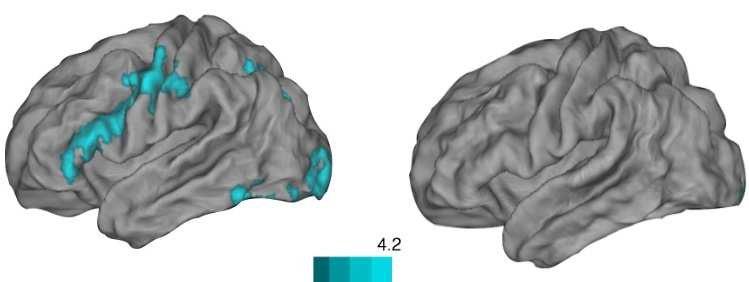
\includegraphics[width=\linewidth]{Seminar Poster/Figures/expected-results-eba-activation.jpg}
}
%....................................................................................
%
%	Block
%
\block[titleleft,roundedcorners=16]{3. Experimental Task}{
	\raggedright
	A finger movement task where (healthy) subjects \textbf{perform better over time}, naturally.
	
	\textbf{Reward} will be \textbf{manipulated} experimentally by visual correct/incorrect feedback.
	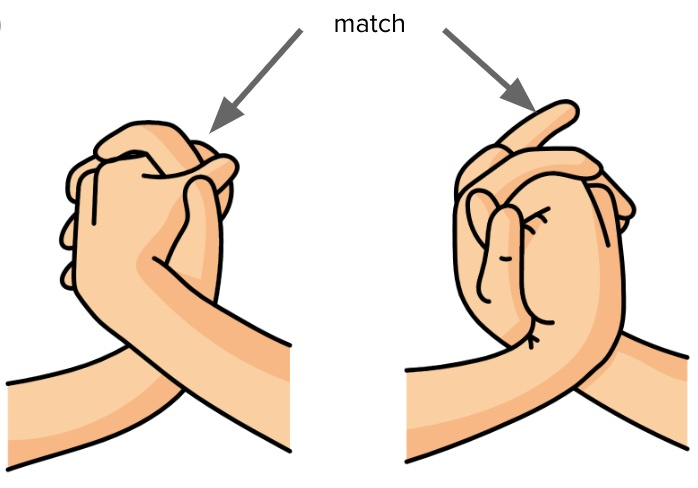
\includegraphics{Seminar Poster/Figures/task-meme.jpg}
}
%..............................................................................................................................................................................................
%
%	CENTER COLUMN
%
\column{0.34}
%....................................................................................
%
% 	Block
%
\block[titleleft,roundedcorners=16]{4. Hypothesis 1}{
	\raggedright
	Hypothesis 1: EBA activation is higher in congruent situation vs non congruent situation (in healthy patients)
 }
%....................................................................................
%
%	Block
%
\block[titleleft,roundedcorners=16]{5. Results H1}{
	\raggedright
}
%..............................................................................................................................................................................................
%
% 	RIGHT COLUMN
%
\column{0.33}
%%....................................................................................
%
%	Block
%
\block[titleleft,roundedcorners=16]{6. Hypothesis 2}{
	\raggedright
	
	}
%....................................................................................
%
%	Block
%
\block[titleleft,roundedcorners=16]{7. Results H2}{
	\raggedright
	
 }
\end{columns} 
%..............................................................................................................................................................................................
%
%	FOOT
%
%....................................................................................
%
%	References
%
\block[titleleft,roundedcorners=16]{}{
\small
\begin{minipage}{0.73\linewidth}
	\nocite{*}
	\bibliographystyle{unsrtnat}
	\bibliography{BibPoster}
 \end{minipage}
%....................................................................................
%
%	Logos
%
\begin{minipage}{0.2\linewidth}
\centering
	
\includegraphics[height=5cm]{Figures/Logo_GitHub}
	
\includegraphics[height=5cm]{Figures/github-link-qr-code}
\end{minipage}
}
%....................................................................................
%
%	My info
%
\note[width=14cm,targetoffsetx=3cm,targetoffsety=3cm,rotate=15]{
	\textbf{Contact information:}\\
	antonio.amaddio@fu-berlin.de
}
\end{document}